\section{Services}
\label{sec:services}
\subsection{Test Services}
\label{sec:testservices}

We can separate services into test and operational services.  Table
\ref{tab:testservers} lists known test services supporting ECH. All of those
below .ie, myechtest.site and my-own.net were setup by the DEfO project.

\tiny
\begin{longtblr} [
        caption = {Test Services with ECH},
        label = {tab:testservers}
    ] {
        colspec = {| l | p{0.7\linewidth} |},
        rowhead = 1
    }
    \hline
        Service Name & Details\\

    \hline
        defo.ie & \url{https://defo.ie/ech-check.php} is often used to check ECH\\
        & ECH keys are rotated hourly, private usable for 3 hours, ECHConfigList in DNS contains only latest public\\

    \hline
        draft-13.esni.defo.ie & different server technology (as listed in Table \ref{tab:servers}) instances on different ports as listed at \url{https://defo.ie/}, e.g., \url{https://draft-13.esni.defo.ie:10413} is served by nginx\\
        & ECH keys are rotated hourly, private usable for 3 hours, ECHConfigList in DNS contains only latest public\\

    \hline
        test.defo.ie & hosts a number of ECH server setups with good and variously bad configurations - see
        \url{https://test.defo.ie/iframes_tests} which describes those and allows a browser to attempt connections to
        each via Iframes\\
        & ECH keys/configs are static for these setups\\

    \hline
        foo.ie & \url{https://foo.ie/ech-check.php} was setup used to check the defo.ie setup was easily replicated\\
        & ECH keys are rotated hourly, private usable for 3 hours, ECHConfigList in DNS contains only latest public\\

    \hline
        my-own.net & this was to test the impact of having the same ECH keys on
        port 443 (\url{https://my-own.net/ech-check.php}) and another port  
        (\url{https://my-own.net:8443/ech-check.php})  - at one point that made a difference to browsers\\
        & ECH keys are rotated hourly, private usable for 3 hours, ECHConfigList in DNS contains only latest public\\

    \hline 
        myechtest.site & this server always treats ECH as if it were GREASE and, in addition
        always returns malformed values in retry-configs to enable some fuzzing of client handling of
        retry-configs\\
        & the ``malformed-ness'' varies randomly, so if testing against this try record the values received as
        we don't (currently) have comprehensive logging of client accesses and the fuzzed values returned\\

    \hline
        tls-ech.dev & \url{https://tls-ech.dev/} was setup by the boringssl developers as a test server that uses
        boringssl\\ 
        & ECH keys/configs seem to be static for this setup\\

    \hline
        Cloudflare & \url{https://cloudflare-ech.com/cdn-cgi/trace} is a test page
           setup by cloudflare that reports on ECH success/failure\\
        & apparently, the server implementation and infrastucrure are part of Cloudflare's normal setup\\
        & a similar test service used to be available at \url{https://crypto.cloudflare.com/cdn-cgi/trace} but
        that was turned off around the time that ECH was re-enabled for Cloudflare customers\\
        & based on one test on 2024-12-09, new ECH keys are published roughly hourly with a 300 second TTL;
            old ECH public values seem usable for approximately 4 or up to 5 hours;
            and the ECHConfigList published in DNS contains only one public value\\

    \hline
        rfc5746.mywaifu.best & this ECH-enabled web page (\url{https://rfc5746.mywaifu.best/}) seems to have been setup 
        as an ECH test site by someone using DEfO artefacts (nginx and documentation) but without any contact
        having happened between the person who set that up and any of the DEfO-project participants\\
        & the person who set this up documented some of that at \url{https://ckcr4lyf.github.io/tech-notes/services/nginx/nginx-ech.html}\\

    \hline
\end{longtblr}
\normalsize

\subsection{Operational Services}

The only operational ECH service we know of is Cloudflare's deployment.
However, that is non-negligible.  Cloudflare earlier enabled ECH but disabled
it soon after in
October 2023~\footnote{\url{https://community.cloudflare.com/t/early-hints-and-encrypted-client-hello-ech-are-currently-disabled-globally/567730}}
as it caused some back-end issues. They then re-enabled ECH in October 2024.
Our understanding of Cloudflare's deployment is that ECH is enabled by 
default for their ``free'' tier customers, but that paying customers have to
take action to enable ECH.

In contrast, non-paying customers are not provided with a control to disable
only ECH - they have to downgrade to TLSv1.2 in order to disable ECH. This
is something that has been seen in recent weeks after the Russian government
started blocking use of ECH to
Cloudflare.~\footnote{\url{https://betanews.com/2024/11/20/encrypted-client-hello-didnt-solve-censorship-but-still-may-have-a-role-to-play/}}

\subsection{Domain Probe Data}

As part of our DEfO test setup, we have a web page where one can enter a host
name and port and a script on our server will check if ECH is enabled for a web
server at the name and port. (That's at
\url{https://test.defo.ie/domainechprobe.php}.) Data is only stored if there is
an HTTPS resource record for the name and port, if there is not we store
nothing. In cases where this is an HTTPS resource record, we only store the
name and port, whether the HTTPS value includes an ``ech='' field, if there is,
whether or not ECH worked using our ECH-enabled curl as the client. We also
store the HTTPS resource record value, unless there are CNAMES or other
kinds of re-direction involved.

We can use this data to get some further insight into services for which ECH
is enabled. For now, we are not publishing the raw data - while data for the most
recent 50 queries is shown on the web page, if we wanted to publish the raw
data, we'd have to enable some form of consent for users, and it's not clear
that'd be a) easy or b) worthwhile. (We currently take no steps to try record
who made which requests to this page.)

Figure \ref{fig:qtimes} shows the (small) numbers of queries made since August
2024. We can see a noticeable uptick in accesses just-before and after Russia
blocked Cloudflare's ECH service. We also see some usage (at least 15 cases) that
appear to indicate some web site owners may be using this service to check
whether or not they have successfully disabled ECH. (The pattern is two quick
accesses to the same name/port, the first of which indicates ECH worked, and
the second that the HTTPS RR no longer contains an ``ech='' value.)

\begin{figure}
	\centering
	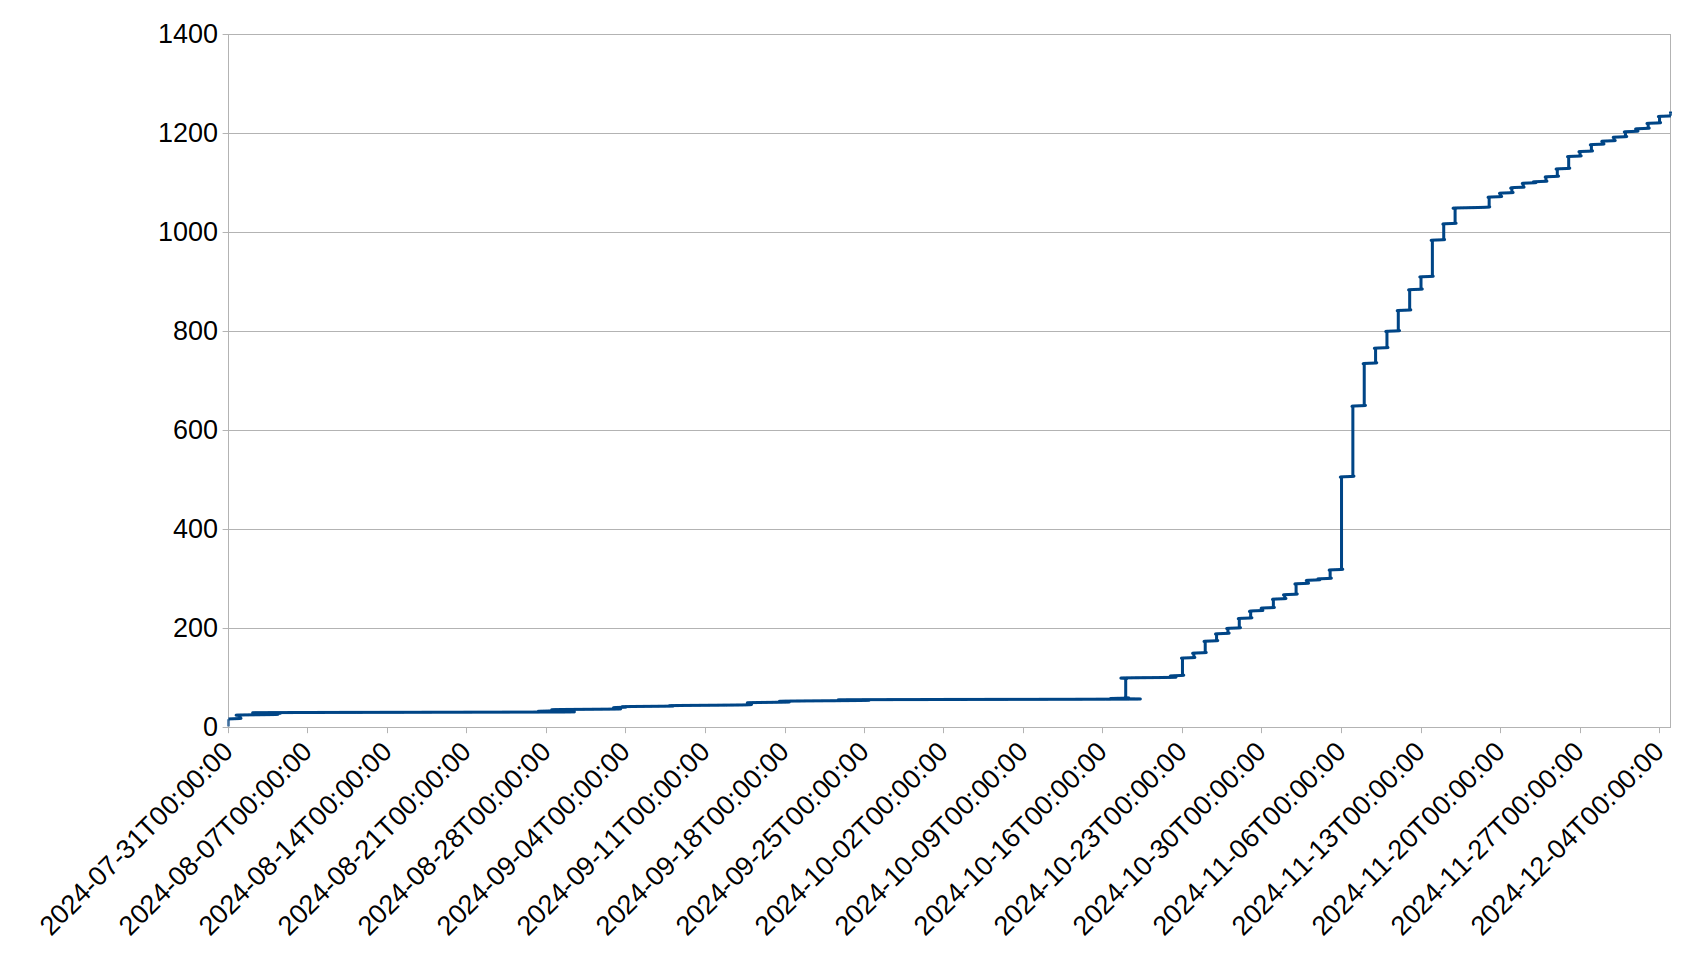
\includegraphics[width=0.8\textwidth,keepaspectratio]{domainprobequeries.png}
		\caption[clustediag]{Cumulative number of queries seen at 
        \url{https://test.defo.ie/domainechprobe.php} versus time. 
        The total number of queries was 1244 as of 2024-12-05.} 
	\label{fig:qtimes}
\end{figure}

The 1244 queries involved 517 unique names (117 of which are under
the ``.ru'' ccTLD). The most commonly queried name is ``youtube.com'' (131 times),
for which ECH is not currently enabled. Some 354 names were only queried 
once, and 86 were queried twice.

Of the 1244 queries, 660 referred to a name that had an ``ech='' in
the relevant HTTPS record, referring to 298 unique names.  Within the 660 HTTPS 
values that contain an ``ech='' value, we see 276 unique ECHConfigList values (4 of which are
corrupt values published for our DEfO test services).  Of the 298 unique
names, 271 seem to be served by Cloudflare (based on the relevant name server
names), 15 relate to test services described in Table \ref{tab:testservers}. At
the time of writing, 9 of the names result in an NXDOMAIN or SERVFAIL
response, 1 seems to correspond to a possible hobbyist site and 2 seem to (now)
be parked domains or part of some advertising campaign. None of those last
3 currently publish an HTTPS record.

So at least for the names entered to our domain probe page, we can seemingly
conclude that Cloudflare have the only operational service at present.
